\documentclass[border=10pt]{standalone}

\usepackage{tikz}
\usepackage{amsfonts}
\usepackage{amssymb}
\usepackage{amsmath}
\usetikzlibrary{arrows,shapes,automata,backgrounds,petri}

\usepackage{lmodern}
\renewcommand{\familydefault}{\sfdefault}

\tikzset{>=latex}

\begin{document}
	
	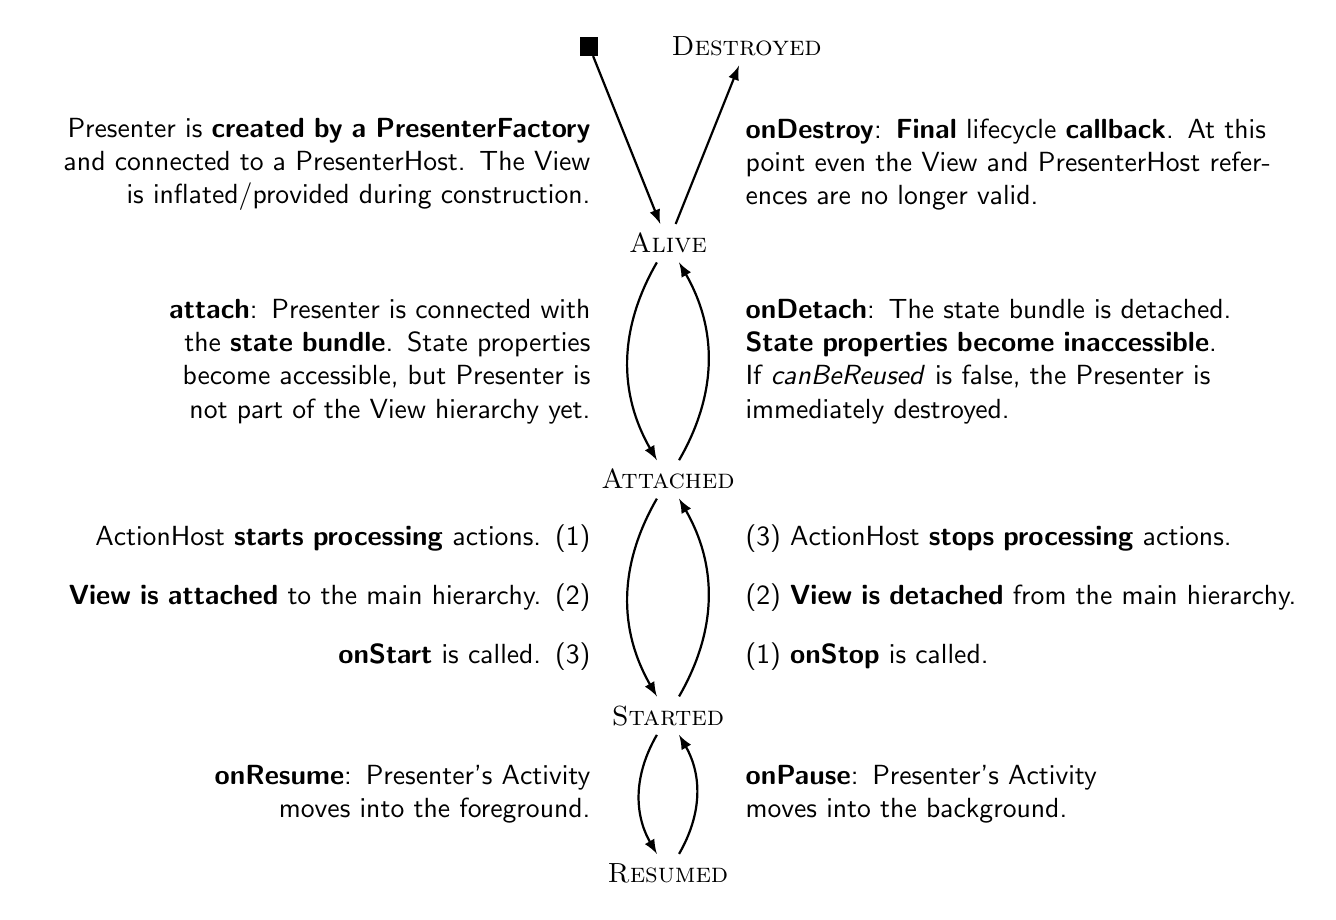
\begin{tikzpicture}[]
	
	\node[](destroyed) at (1,2.5) {\textsc{Destroyed}};

	\node[fill=black](init) at (-1,2.5) {};
	
	\node[](alive) at (0,0) {\textsc{Alive}};
	
	\node[](attached) at (0, -3) {\textsc{Attached}};
	
	\node[](started) at (0, -6) {\textsc{Started}};
	
	\node[](resumed) at (0, -8) {\textsc{Resumed}};
	
	% Descriptions

	\node[text width=20em, align=right](constructor) at (-4.5, 1) { Presenter is \textbf{created by a \mbox{PresenterFactory}} and connected to a PresenterHost. The View is inflated/provided during construction. };
	
	\node[text width=20em](onDestroy) at (4.5, 1) { \textbf{onDestroy}: \textbf{Final} lifecycle \textbf{callback}. At this point even the View and PresenterHost references are no longer valid. };
	
	\node[text width=20em, align=right](attach) at (-4.5, -1.5) { \textbf{attach}: Presenter is connected with the \textbf{state bundle}. State properties become accessible, but Presenter is not part of the View hierarchy yet. };
	
	\node[text width=20em](onDetach) at (4.5, -1.5) { \textbf{onDetach}: The state bundle is detached. \textbf{State properties become inaccessible}. If \emph{canBeReused} is false, the Presenter is \mbox{immediately} destroyed. };
	
	\node[text width=20em, align=right](onStart-1) at (-4.5, -3.75) { ActionHost \textbf{starts processing} actions. (1) };

	\node[text width=20em, align=right](onStart-2) at (-4.5, -4.5) { \textbf{View is attached} to the main hierarchy. (2) };
	
	\node[text width=20em, align=right](onStart-3) at (-4.5, -5.25) { \textbf{onStart} is called. (3) };
	
	\node[text width=20em](onStop-3) at (4.5, -3.75) { (3) ActionHost \textbf{stops processing} actions. };
	
	\node[text width=20em](onStop-2) at (4.5, -4.5) { (2) \textbf{View is detached} from the main hierarchy. };
	
	\node[text width=20em](onStop-1) at (4.5, -5.25) { (1) \textbf{onStop} is called. };
	
	\node[text width=20em, align=right](onResume) at (-4.5, -7) { \textbf{onResume}: Presenter's \mbox{Activity} moves into the foreground. };

	\node[text width=20em](onPause) at (4.5, -7) { \textbf{onPause}: Presenter's Activity \\ moves into the background. };
	
	% Arrows
	
	\draw [->=stealth, thick] (alive) to (destroyed);
	\draw [->=stealth, thick] (init) to (alive);
	
	\draw [->=stealth, thick, bend right] (alive) to (attached);
	\draw [->=stealth, thick, bend right] (attached) to (alive);

	\draw [->=stealth, thick, bend right] (attached) to (started);
	\draw [->=stealth, thick, bend right] (started) to (attached);

	\draw [->=stealth, thick, bend right] (started) to (resumed);
	\draw [->=stealth, thick, bend right] (resumed) to (started);
		
	\end{tikzpicture}
	
\end{document}